\documentclass[11pt]{article}

\usepackage{amsmath,amssymb}	% for mathematical notation
\usepackage{float} 				% put things exactly where I tell you!
\usepackage[utf8]{inputenc} 	% can we has UTF-8, plox
\usepackage{listings}           % for embedded code
\usepackage{graphicx}           % for pretty pictures

\title%
{%
	{\large Miniprojekt}\\
	Biludlejning
}

\author%
{%
	Andreas Dall Løfgren\\
	\and
	Stine Knarkegaard Andersen\\
	\and
	Chris Dan Justesen\\
}

\begin{document}
\maketitle
\tableofcontents
\pagebreak

\section*{Systemudvikling}
\subsection*{Use-case}
\begin{figure}
  \centering
  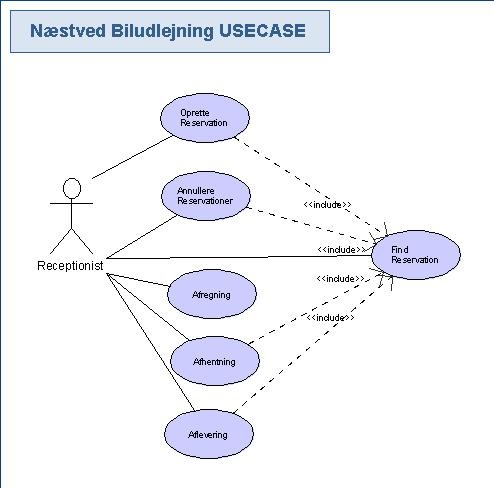
\includegraphics[width=10cm]{Naestved_Biludlejning_USECASE.jpeg}
  \caption{Brugsmønstre}
  \label{fig:Use-case diagram}
\end{figure}

\begin{tabular}{ l | p{10cm} }
Oprette reservation & Oprettelse af reservationer ved indtastning af kundeoplysninger og biloplysninger. Laver en lejekontrakt. \\ \hline
Annullere reservationer & Annullering af reservation, hvis en reservation skal slettes. \\ \hline
Afregning & Den samlede afregning for lejen. \\ \hline
Afhentning & Kunden afhenter bilen. Bilens korte kilometer skal noteres.\\ \hline
Aflevering & Aflevering af bilen. Mængden af benzin og det kørte antal kilometer skal noteres. \\ \hline
Find reservation & Søgning af reservationer baseret på navn, dato, cpr-nummer, eller andet.
\end{tabular}\\

Af disse brugsmønstre da er oprettelse af reservationer den vigtigste, da den er påkrævet for at de andre fungerer. Alle funktioner undtagen afregning gå ind og ændrer på lejekontrakten, derfor inkluderer de Find reservation, da den bliver brugt til at søge i reservationerne.\\

Successcenarie for Oprettelse af reservation:
\begin{enumerate}
\item Kunden siger hvilken periode og prisgruppe han er interesseret i.
\item En liste over ledige biler kommer frem.
\item Man kommer til kundeoplysninger, der bliver skrevet ind.
\item Den færdige lejekontrakt bliver lavet og kan eventuelt printes.\\
\end{enumerate}

Specialscenarie for Oprettelse af reservation:
\begin{enumerate}
\item Kunden siger hvilken periode og prisgruppe han er interesseret i.
\item Hvis der ikke er nogle ledige biler i den prisgruppe, da vil der ikke komme nogle biler frem.
\end{enumerate}

Løsningen er at tilbyde en bil fra en anden prisgruppe. \\

\subsection*{Domænemodel}
\begin{figure}
  \centering
  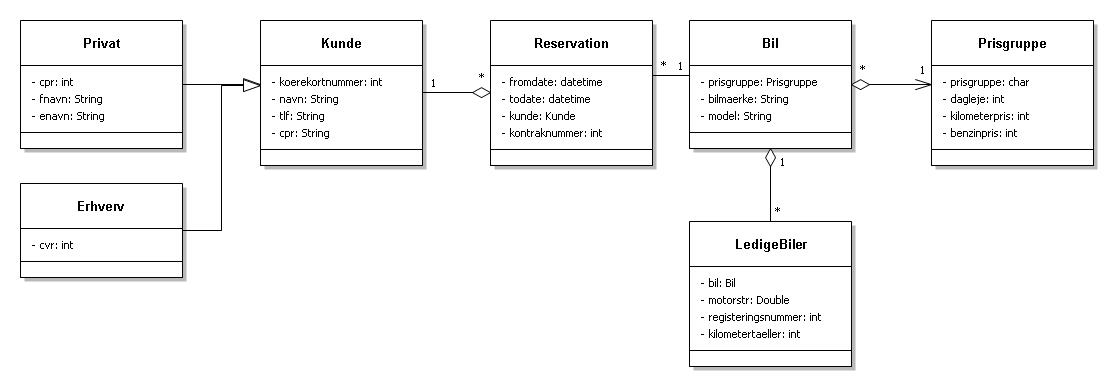
\includegraphics[width=15cm]{CLASSDIAGRAM.jpg}
  \caption{Domænemodel}
  \label{fig:Domaenemodel}
\end{figure}

I vores domænemodel har vi en generaliseret kundeklasse til en privatkunde og erhvervskunde, da man skal registrere forskellige oplysninger til hver.\\\\
Reservationsklassen bruger et kundeobjekt til at blive oprettet og henter oplysninger fra bilklassen. Den har også en til- og fra-dato.\\\\
Bilklassen bruger et prisgruppeobjekt til at blive oprettet.\\\\
Prisgruppe indeholder de forskellige kategorier for bilerne og indeholder også alle priserne (dagleje, kilometerpris og benzinpris).\\\\
Klassen LedigeBiler bruges til at holde styr på de fysiske udgaver af bilerne og viser hvilke der er ledige for udlejning. Den har oplysninger om den enkelte bil. Den bruger et bilobjekt til at blive oprettet.

\section*{Programmering}
\subsection*{Database}
\begin{figure}
  \centering
  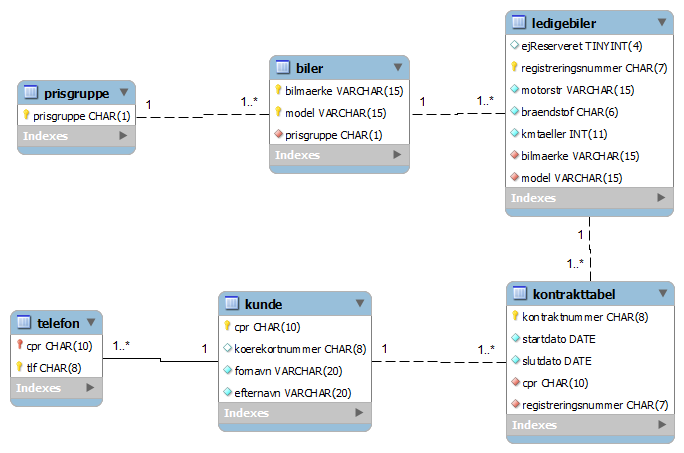
\includegraphics[width=15cm]{ER-diagram.png}
  \caption{ER-diagram}
  \label{fig:ER-diagram}
\end{figure}

Vores database er normaliseret til tredje normalform og indeholder seks tabeller. Prisgruppe indeholder kun prisgruppen. Bil indeholder oplysninger om bilerne. Ledigebiler indeholder oplysninger om den enkelte bil. Kunde indeholder alle kundeoplysningerne og kontrakttabel indeholder alle kontraktoplysningerne. Telefon er en flerværdiattribut, der har fået sin egen tabel.

\subsection*{Klassediagram}
\begin{figure}
  \centering
  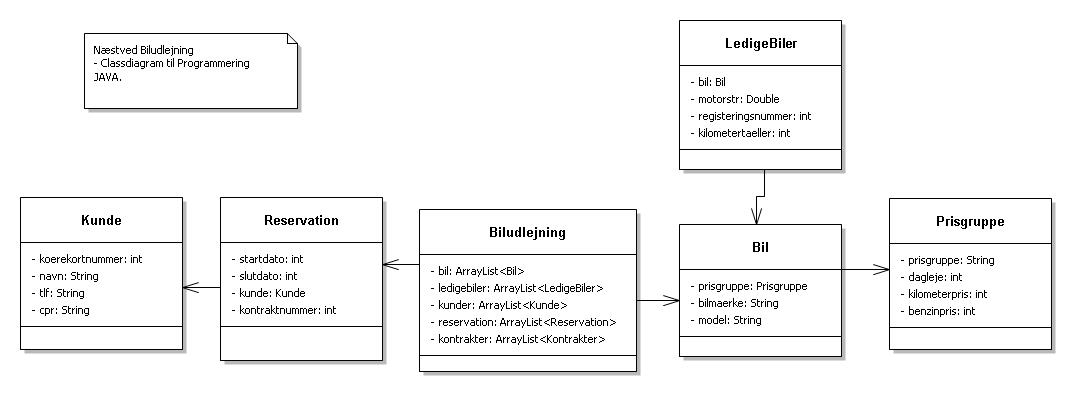
\includegraphics[width=15cm]{Classdiagram_prog.jpg}
  \caption{Klassediagram}
  \label{fig:Klassediagram}
\end{figure}

Vores klassediagram, der viser hvad programmet indeholder:\\
Prisgruppeklassen indeholder priser og bilkategorier. Bilklassen indeholder prisgruppe og oplysniinger om bilerne. De ledige biler har en klasse for sig selv, der bruger bilklassen. Kundeklassen indeholder alle oplysninger om kunden. Reservationsklassen bruger kundeklassen til at oprette en reservation og Det hele ligger i arraylister i biludlejningsklassen.

\subsection*{Kode}
Modelklasserne består udelukkende af gettere og settere.\\\\
GUI'en er bygget op med tabs for de forskellige skærmvinduer. Man kan fra forsiden oprette eller finde reservationer.\\\\
Hvis man vil oprette en reservation, da skal man først vælge en periode og en prisgruppe, så kommer en liste af ledige biler. Efter man har valgt en bil skal man trykke næste og indtaste kundeoplysninger og bagefter opretter man kunden og så har man den færdige lejekontrakt.\\\\
Hvis man vil søge efter en reservation, kan man søge efter flere parametre og man vil få en tabel med søgeresultaterne.

\end{document}